\documentclass{amsart}

\usepackage{tikz}

%\tikzstyle{every node}=[circle, draw, fill=black,
%                        inner sep=0pt, minimum width=2pt]

%\tikzstyle{every node}=[circle, draw, fill=black]

\tikzstyle{cr}=[radius=0.1]
\tikzstyle{ln}=[fill, dashed]
												
\begin{document}
	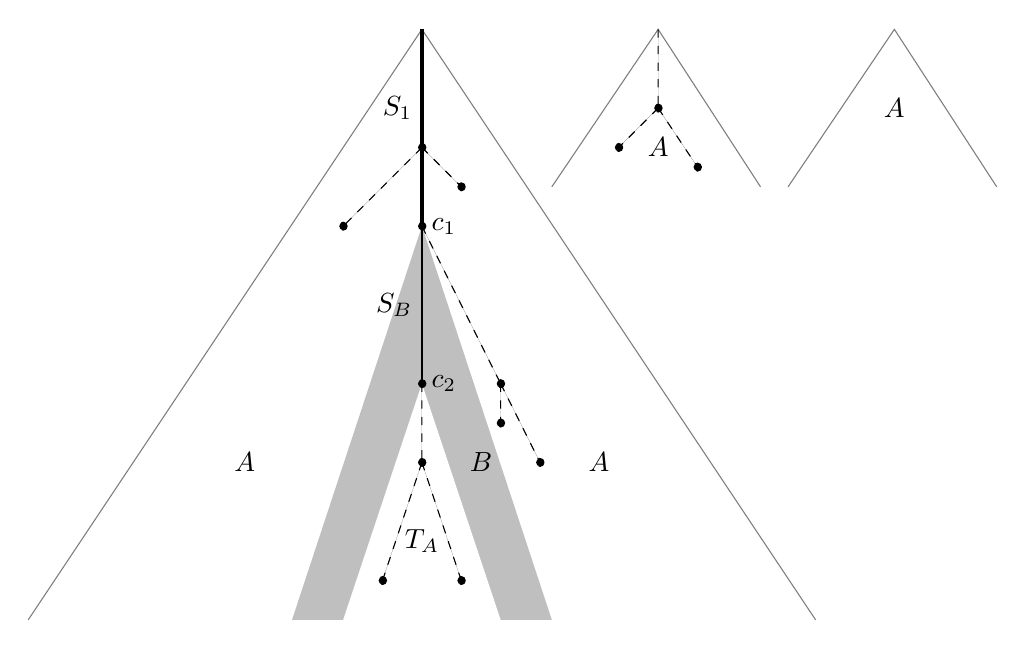
\begin{tikzpicture}[scale=.5]
		%\path [fill=blue] (-10,-15) -- (0,0) -- (10,-15);
		%\path [fill=orange] (3.3,-4) -- (6,0) -- (8.6,-4);
		%\path [fill=brown] (9.3,-4) -- (12,0) -- (14.6,-4);
		
		\path [fill=lightgray] (-3.3,-15) -- (0,-5) -- (3.3, -15);
		%\path [fill=red] (3.3,-15) -- (0,-5) -- (6.6,-15);
		%\path [fill=cyan] (-3.3,-15) -- (0,-5) -- (-6.6,-15);
		\path [fill=white] (0,-9) --  (-2,-15) -- (2, -15);

		\draw [gray] (0,0) -- (-10,-15);
		\draw [gray] (0,0) -- (10, -15);

		%\draw [gray] (0,-5) -- (-6.6,-15);
		%\draw [gray] (0,-5) -- (6.6, -15);

		%\draw [gray] (0,-5) -- (-3.3,-15);
		%\draw [gray] (0,-5) -- (3.3, -15);

		%\draw [gray] (0,-9) -- (-2,-15);
		%\draw [gray] (0,-9) -- (2, -15);
		
		\draw [gray] (3.3,-4) -- (6,0) -- (8.6,-4);
		\draw [gray] (9.3,-4) -- (12,0) -- (14.6,-4);
		
		\draw[ln] (0,0) -- (0,-3) circle [cr] node{};
		\draw[ln] (0,-3) --(1,-4) circle [cr] node{};
		\draw[ln] (0,-3) --(-2,-5) circle [cr] node{};
		
		\draw[ln] (0,-3) --(0,-5) circle [cr] node[right]{$c_1$};

		\draw[ln] (0,-5) --(0,-9) circle [cr] node[right]{$c_2$};
		
		\draw[ln] (0,-9) --(0,-11) circle [cr] node{};
		\draw[ln] (0,-11) --(-1,-14) circle [cr] node{};
		\draw[ln] (0,-11) --(1,-14) circle [cr] node{};

		\draw[ln] (0,-5) --(2,-9) circle [cr] node{};
		\draw[ln] (2,-9) --(2,-10) circle [cr] node{};
		\draw[ln] (2,-9) --(3,-11) circle [cr] node{};
				
		
		\draw[ln] (6,0) -- (6,-2) circle [cr] node{};
		\draw[ln] (6,-2) --(7,-3.5) circle [cr] node{};
		\draw[ln] (6,-2) --(5,-3) circle [cr] node{};
		
		\draw [very thick] (0,0) -- (0,-5);
		\draw [thick] (0,0) -- (0,-9);
		\node [left] at (0, -2) {$S_1$};
		\node [left] at (0, -7) {$S_B$};

		\node at (1.5, -11) {$B$};
		
		\node at (4.5, -11) {$A$};
		\node at (-4.5, -11) {$A$};
		%\node at (-.5, -2) {$A$};
		
		\node at (0, -13) {$T_A$};
		
		\node at (6,-3) {$A$};
		\node at (12,-2) {$A$};
		
		
	\end{tikzpicture}
\end{document}